\documentclass{beamer}

\usepackage{graphicx}
\usepackage{mathtools}
\usepackage{mathrsfs}

%Information to be included in the title page:
\title{Cause-Effect Models}
\author{Congyuan Duan}
%\institute{School of Mathematics, Sun Yat-sen University}



\begin{document}

\frame{\titlepage}

\begin{frame}
    \frametitle{Contents}
    \tableofcontents
\end{frame}

\section{Structural Causal Models}

\begin{frame}
    \frametitle{Contents}
    \tableofcontents[currentsection]
\end{frame}

\begin{frame}
    \frametitle{Definition}
    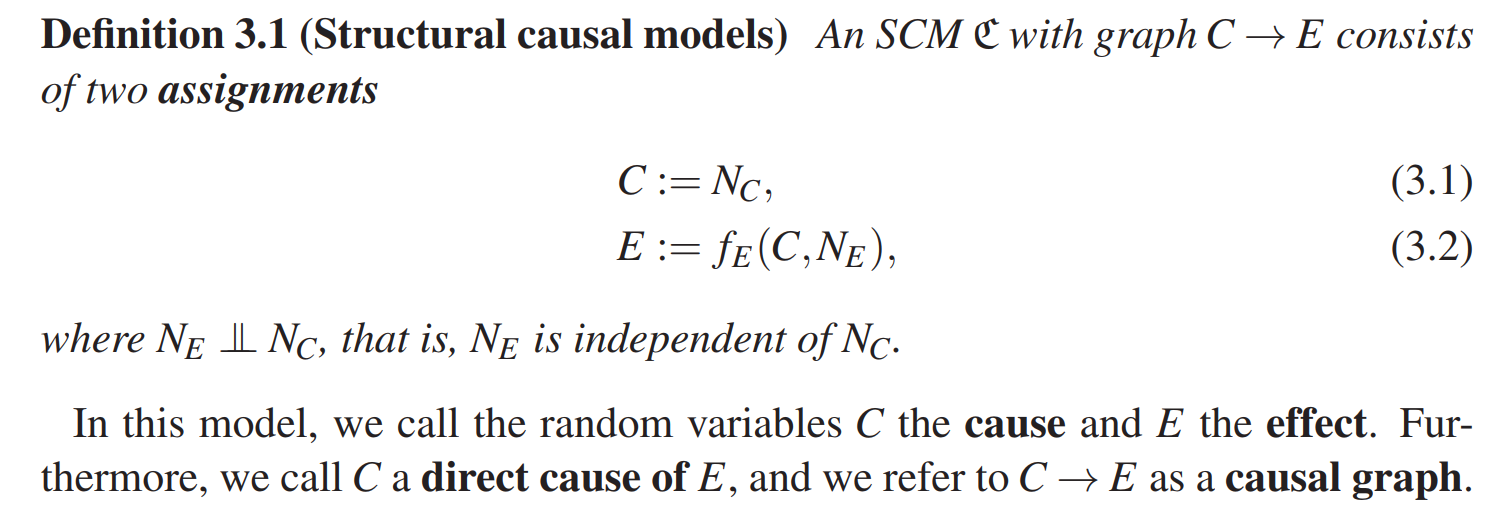
\includegraphics[scale=0.55]{fig1.png} 
\end{frame}

\begin{frame}
    \frametitle{Graphical Representation}
    Formally, a structural causal model consists of two sets of variables $U$ and $V$, and a set of
    functions $f$ that assigns each variable in $V$ a value based on the values of the other variables
    in the model. A variable $X$ is a direct cause of a variable $Y$ if $X$ appears in the function that 
    assigns $Y$'s value. \\
    \begin{itemize}
        \item[$\bullet$] The variables in U are called \textbf{exogenous variables}, meaning that they are external to
        the model; we choose not to explain how they are caused.
        \item[$\bullet$] The variables in V are \textbf{endogenous variables}. Every endogenous variable in a model is a 
        descendant of at least one exogenous variable. 
    \end{itemize}
    Exogenous variables cannot be descendants of any other variables.
\end{frame}

\begin{frame}
    \frametitle{Example: College Acceptance} 
    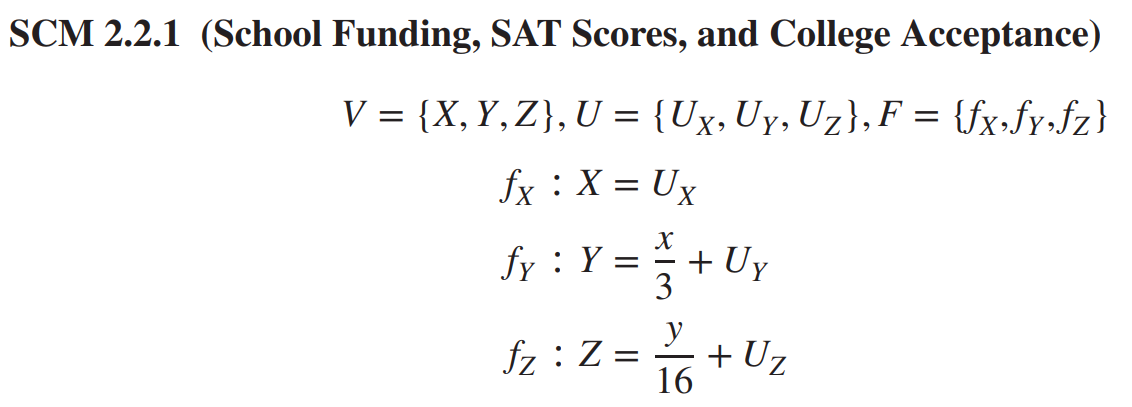
\includegraphics[scale=0.6]{fig2.png}
    \centering{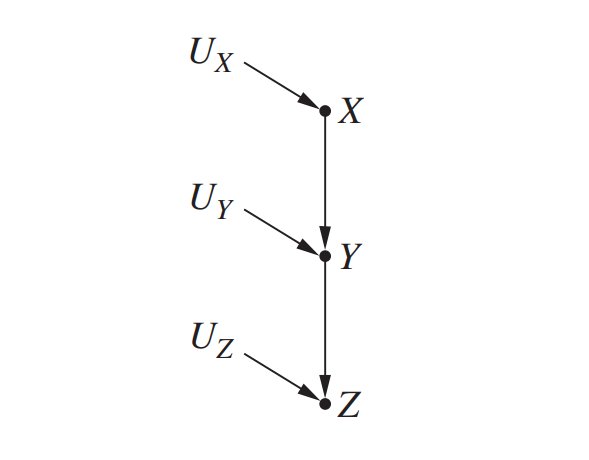
\includegraphics[scale=0.6]{fig3.png}}
\end{frame}


\section{Interventions}

\begin{frame}
    \frametitle{Contents}
    \tableofcontents[currentsection]
\end{frame}

\begin{frame}
    \frametitle{Cause-effect interventions}
    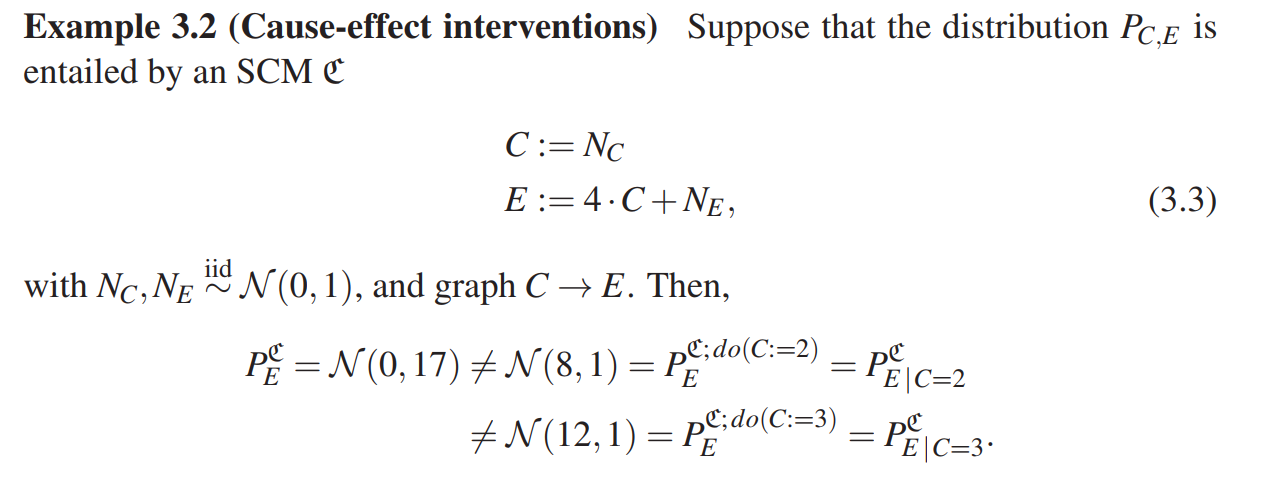
\includegraphics[scale=0.6]{fig9.png}
    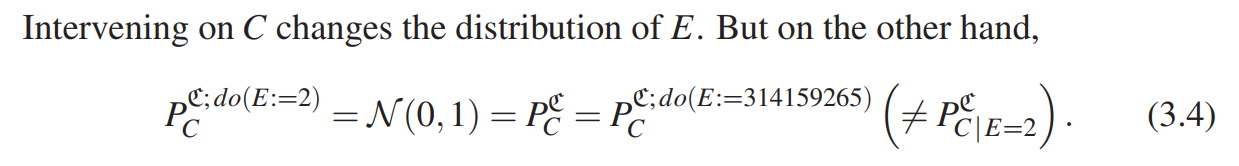
\includegraphics[scale=0.6]{fig10.png}
\end{frame}

\begin{frame}
    \frametitle{Graphical Representation}
    When we intervene on a variable, we remove all edges directed into it.
    \begin{figure}[htbp]
        \centering
        \begin{minipage}[t]{0.48\textwidth}
        \centering
        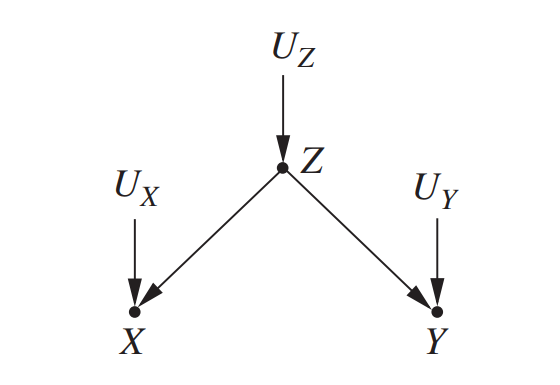
\includegraphics[scale=0.6]{fig11.png}
        \end{minipage}
        \begin{minipage}[t]{0.48\textwidth}
        \centering
        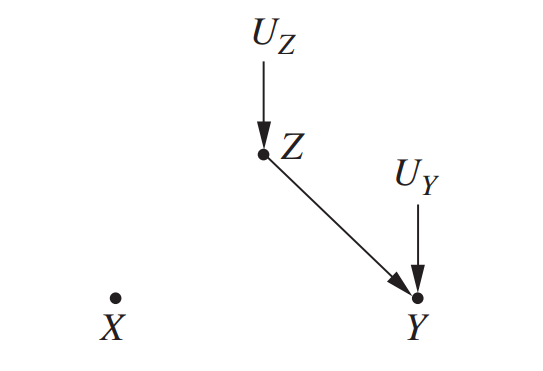
\includegraphics[scale=0.6]{fig12.png}
        \end{minipage}
    \end{figure}
\end{frame}

\begin{frame}
    \frametitle{Interventions and Conditioning}
    $p(y|do(x))$ and $p(y|x)$ are not generally the same. 
    \begin{itemize}
        \item[$\bullet$] Conditioning $p(y|x)$: What is the distribution of $Y$ given that I \textbf{observe} 
        variable $X$ takes value $x$.
        \item[$\bullet$] Interventions $p(y|do(x))$: What is the distribution of $Y$ if I were to \textbf{set} 
        the value of $X$ to $x$. 
    \end{itemize}
    In summary, $y$ and $x$ are statistically dependent and therefore seeing $x$ allows us to predict the value 
    of $y$, but $y$ is not caused by $x$ so setting the value of $x$ won't effect the distribution of $y$. 
\end{frame}

\begin{frame}
    \frametitle{Interventions and Conditioning} 
    We are interested in $p(y|x)$. In the simple supervised learning case, we can build a model $q(y|x;\theta)$ from the 
    training data to approximate $p(y|x)$. \\
    \centering{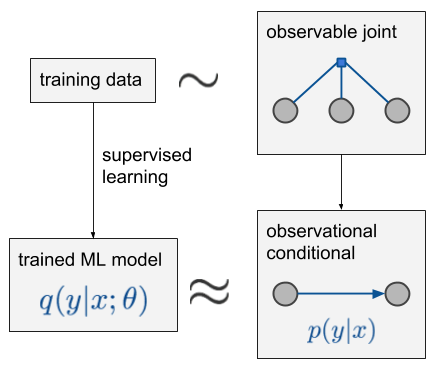
\includegraphics[scale=0.4]{fig5.png}}
\end{frame}

\begin{frame}
    \frametitle{Interventions and Conditioning} 
    What if we're actually interested in $p(y|do(x))$ rather than $p(y|x)$? The intervention joint is a joint distribution over 
    the same domain as $p$ but it's a different distribution. \\
    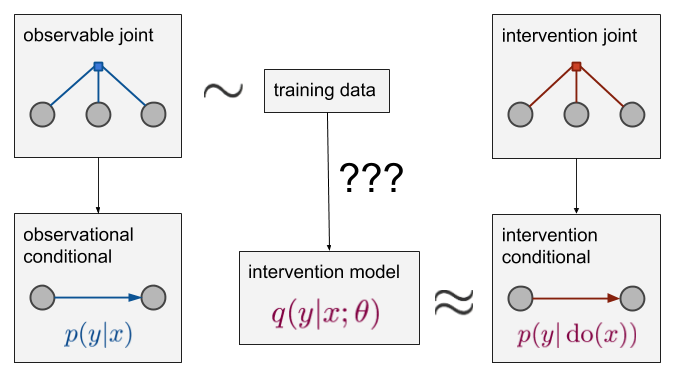
\includegraphics[scale=0.4]{fig6.png} \\
    We want to estimate the red conditional $p(y|do(x))$ from the blue joint.
\end{frame}

\begin{frame}
    \frametitle{Interventions and Conditioning} 
    If we know about the causal structure, we can establish a connection between the blue and the red joints. 
    Then we can emulate the effect of intervention by deleting all edges that lead into  nodes in a $do$ operator. \\
    \centering{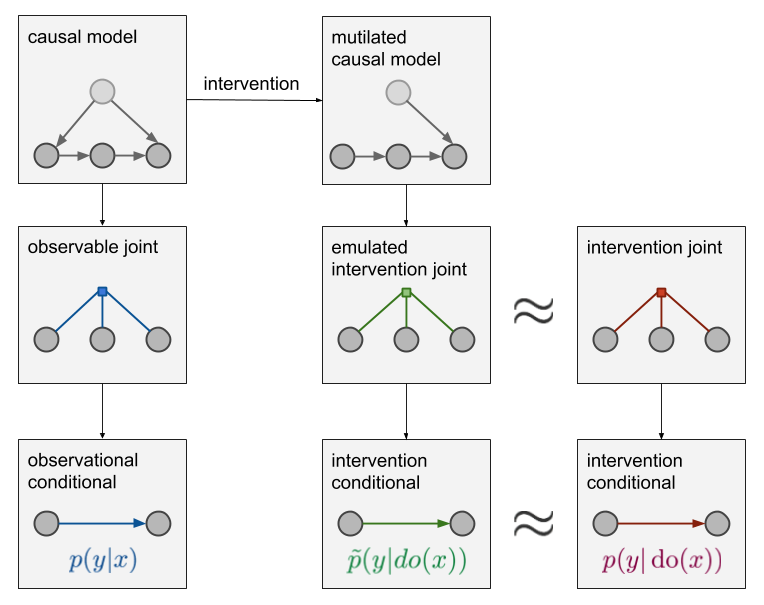
\includegraphics[scale=0.3]{fig7.png}}
\end{frame}

\begin{frame}
    \frametitle{Interventions and Conditioning} 
    Do-calculus allows us to massage the green conditional distribution 
    until we can express it in terms of various marginals, conditionals and expectations under the blue distribution. \\
    \centering{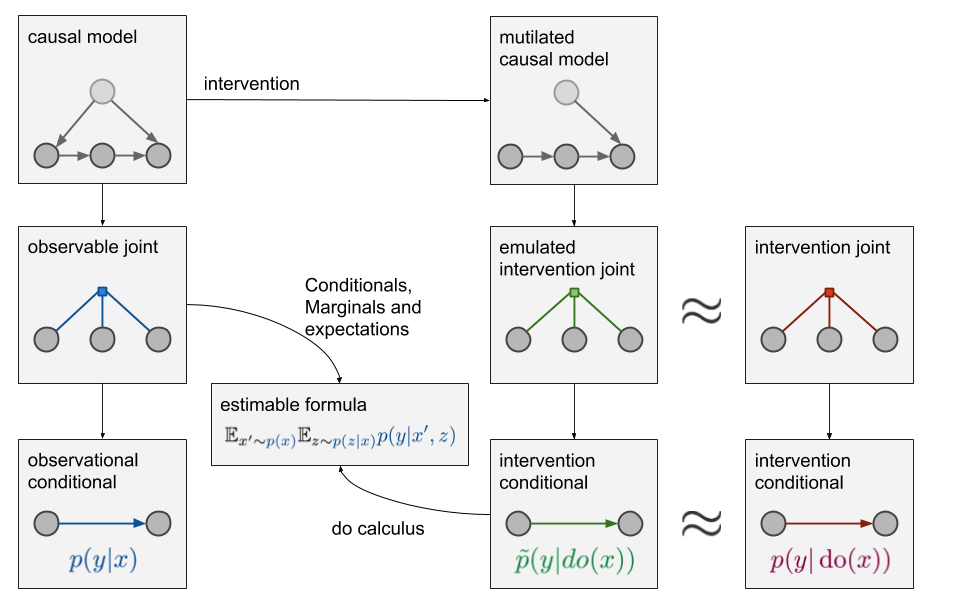
\includegraphics[scale=0.3]{fig8.png}}
\end{frame}

\section{Counterfactuals}

\begin{frame}
    \frametitle{Contents}
    \tableofcontents[currentsection]
\end{frame}

\begin{frame}
    \frametitle{Example: Eye disease} 
    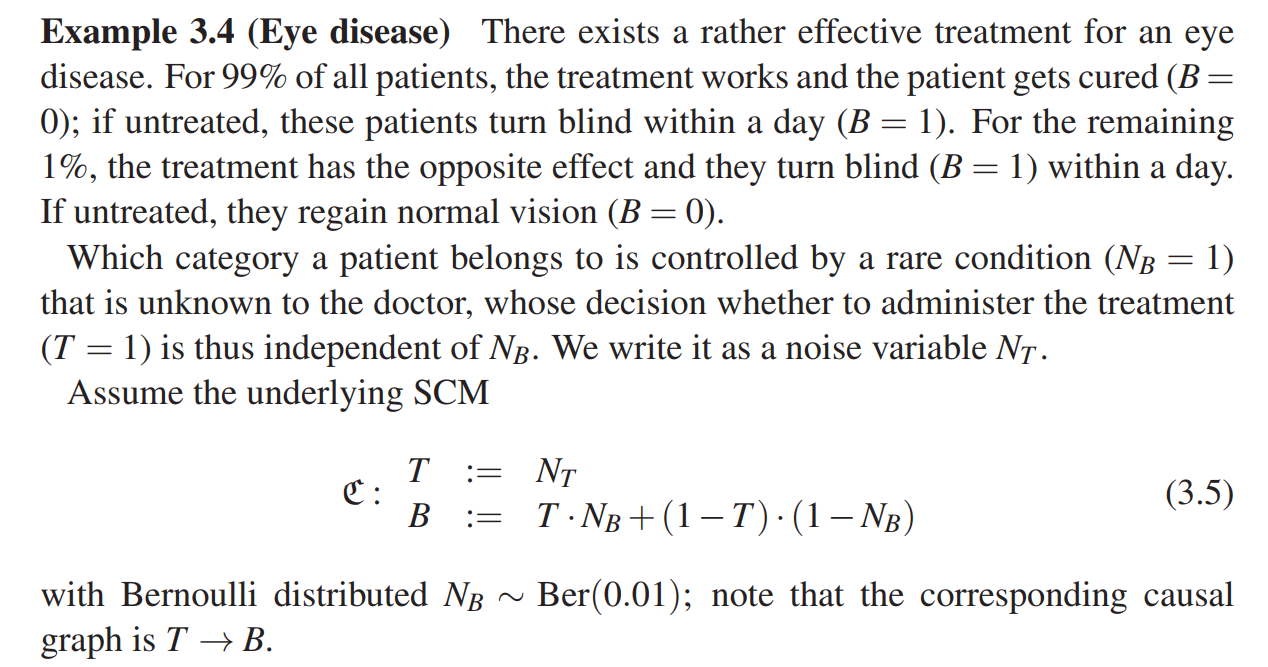
\includegraphics[scale=0.6]{fig13.png} \\
    A specific patient with poor eyesight comes to the hospital and goes blind ($B=1$) after the doctor administers 
    the treatment ($T=1$). \textbf{“What would have happened had the doctor administered treatment $\textbf{T = 0}$?”}
\end{frame}

\begin{frame}
    \frametitle{Steps in Computing Counterfactuals}
    \begin{itemize}
        \item[$\bullet$] Every assignment $U = u$ corresponds to a single member
        or "unit" in a population, or to a "situation" in nature.
        \item[$\bullet$] Since we have gleaned knowledge about the previously unknown noise variables for the given individual, 
        we update the noise distributions.
    \end{itemize} 
    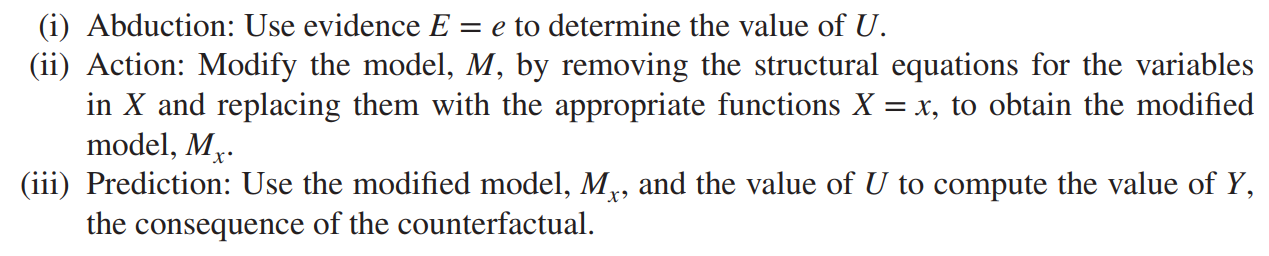
\includegraphics[scale=0.6]{fig14.png}
    Remark: Nondeterministic Counterfactuals.
\end{frame}


\begin{frame}
    \frametitle{Interventions and Counterfactuals} 
    \begin{itemize}
        \item[$\bullet$] Interventions: If I take aspirin, will my headache be cured?(population, 
        new distribution)
        \item[$\bullet$] Counterfactuals: Was it the aspirin that stopped my headache?(individual)
    \end{itemize}
\end{frame}

\begin{frame}
    \frametitle{Interventions and Counterfactuals} 
    Consider the model
    \begin{align*}
        X=U_1\quad Z=aX+U_2\quad Y=bZ
    \end{align*}
    Let $X=1$ stand for having a college education, $U_2=1$ for having professional experience, $Z$ for the level of skill needed
    for a given job, and $Y$ for salary. Suppose our aim is to compute $E[Y_{X=1}|Z=1]$, which stands for the expected salary of individuals 
    with skill level $Z = 1$, had they received a college education.
    
\includegraphics[scale=0.6]{fig4.png}
\end{frame}

\begin{frame}
    \frametitle{Interventions and Counterfactuals} 
    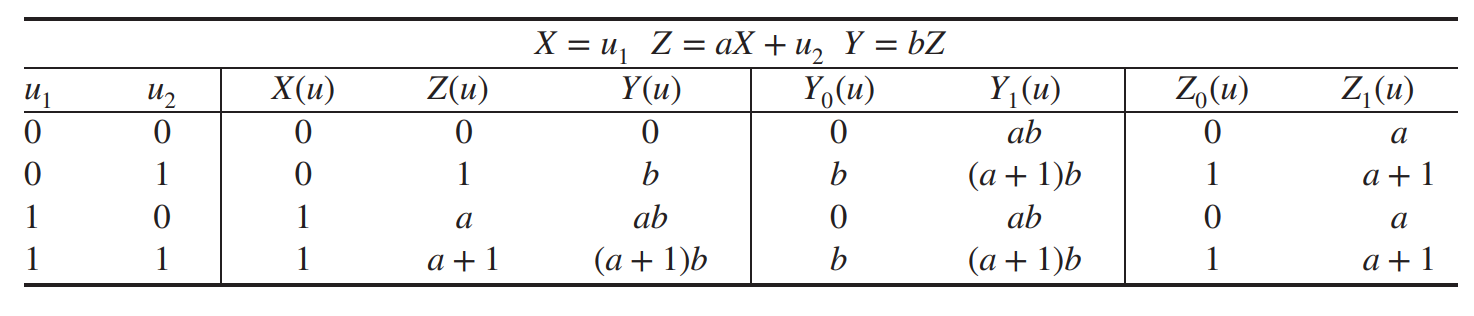
\includegraphics[scale=0.55]{fig15.png}
    \leftline{Using this table, we can verify that} 
    \centering{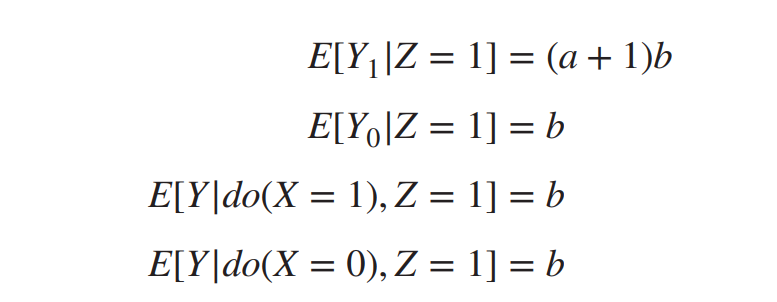
\includegraphics[scale=0.6]{fig16.png}}
    \leftline{and} \\
    \centering{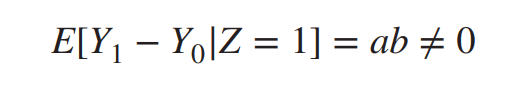
\includegraphics[scale=0.6]{fig17.png}}
\end{frame}


\section{Canonical Representation of Structural Causal Models}

\begin{frame}
    \frametitle{Contents}
    \tableofcontents[currentsection]
\end{frame}

\begin{frame}
    \frametitle{Reference} 
    https://www.inference.vc/untitled/ \\
    Pearl J, Glymour M, Jewell N P. Causal inference in statistics: A primer[M]. John Wiley \& Sons, 2016. \\

\end{frame}


\end{document}
